\let\negmedspace\undefined
\let\negthickspace\undefined
\documentclass[journal]{IEEEtran}
\usepackage[a5paper, margin=10mm, onecolumn]{geometry}
%\usepackage{lmodern} % Ensure lmodern is loaded for pdflatex
\usepackage{tfrupee} % Include tfrupee package

\setlength{\headheight}{1cm} % Set the height of the header box
\setlength{\headsep}{0mm}  % Set the distance between the header box and the top of the text

\usepackage{gvv-book}
\usepackage{gvv}
\usepackage{cite}
\usepackage{amsmath,amssymb,amsfonts,amsthm}
\usepackage{algorithmic}
\usepackage{graphicx}
\usepackage{textcomp}
\usepackage{xcolor}
\usepackage{txfonts}
\usepackage{listings}
\usepackage{enumitem}
\usepackage{mathtools}
\usepackage{gensymb}
\usepackage{comment}
\usepackage[breaklinks=true]{hyperref}
\usepackage{tkz-euclide} 
\usepackage{listings}
% \usepackage{gvv}                                        
\def\inputGnumericTable{}                                 
\usepackage[latin1]{inputenc}                                
\usepackage{color}                                            
\usepackage{array}                                            
\usepackage{longtable}                                       
\usepackage{calc}                                             
\usepackage{multirow}                                         
\usepackage{hhline}                                           
\usepackage{ifthen}                                           
\usepackage{lscape}
\begin{document}

\bibliographystyle{IEEEtran}
\vspace{3cm}

\title{9.3.23}
\author{EE24BTECH11021 - Eshan Ray}

% \maketitle
% \newpage
% \bigskip
{\let\newpage\relax\maketitle}

\renewcommand{\thefigure}{\theenumi}
\renewcommand{\thetable}{\theenumi}
\setlength{\intextsep}{10pt} % Space between text and floats




\textbf{Question: }\\
Find the area bounded by the ellipse $x^2 + 4y^2 = 16$ and the ordinates $x = 0$ and $x = 2$, using integration.\\
\solution {
\begin{table}[h!]    
  \centering
  \begin{tabular}[12pt]{ |c| c|}
    \hline
        \textbf{Variable}  & \textbf{Description} \\
    \hline
        $\vec{B}$$\brak{-4,0}$ &  coordinates of first point  \\
    \hline 
        $\vec{C}$$\brak{10,0}$ & coordinates of second point \\
    \hline
        $\vec{A}$& Equidistant point of $\vec{B}$ and $\vec{C}$ on $X$ axis \\  
    \hline
         
\end{tabular}

  \caption{Input parameters}
  \label{tab1.1.9.2}
\end{table}
\\
The point of intersection of the line with the ellipse is $x_i=h+k_i m$,\\
where,$k_i$ is a constant and is calculated as follows:-
$$k_i=\frac{1}{m^\top Vm}\brak{-m^\top \brak{Vh+u}\pm \sqrt{\sbrak{m^\top \brak{Vh+u}}^2-g\brak{h}\brak{m^\top Vm}}}$$\\
\begin{multline}
     k_i =\frac{1}{\myvec{0&1}\myvec{4&0\\0&16}\myvec{0\\1}}\brak{-\myvec{0&1}\brak{\myvec{4&0\\0&16}\myvec{2\\0}+0}\pm \\
     \sqrt{\sbrak{\myvec{0&1}\brak{\myvec{4&0\\0&16}\myvec{2\\0}+0}}^2-g\brak{h}\brak{\myvec{0&1}\myvec{4&0\\0&16}\myvec{0\\1}}}}
\end{multline}
We get,\\
$$k_i= \sqrt{3},-\sqrt{3}$$
\begin{align}
     x_1&=\myvec{2\\0}+\brak{\sqrt{3}}\myvec{0\\1}\\
    \implies x_1 &=\myvec{2\\0} + \myvec{0\\ \sqrt{3}}\\
    \implies x_1 &=\myvec{2\\ \sqrt{3}}\\
    x_2 &=\myvec{2\\0}+\brak{-\sqrt{3}}\myvec{0\\1}\\
    \implies x_2&=\myvec{2\\0}+\myvec{0\\ -\sqrt{3}}\\
    \implies x_2&=\myvec{2\\-\sqrt{3}}
\end{align}
$\therefore$ The bounded area is given by:-
\begin{align}
   Area &= 2\int_{0}^{2} \frac{\sqrt{16-x^2}}{2} \,dx \\
  \implies Area &= \int_{0}^{2} \sqrt{16-x^2} \,dx \\
   \brak{Substituting,x=4\sin{\theta}} \\
   \implies dx&=4\cos{\theta}d\theta\\
   \implies Area&=\int_{0}^{\frac{\pi}{6}} \sqrt{16-\brak{4\sin{\theta}}^2} \,4\cos{\theta}d\theta \\
   \implies &=16\int_{0}^{\frac{\pi}{6}} \sqrt{1-\sin^2{\theta}} \,\cos{\theta}d\theta \\
   \implies &=16\int_{0}^{\frac{\pi}{6}} \cos^2{\theta} \,d\theta \\
   \implies &=16\int_{0}^{\frac{\pi}{6}} \frac{\brak{1+\cos{2\theta}}}{2} \,d\theta \\
   \implies &=8\brak{\sbrak{\theta}\limits_{0}^{\frac{\pi}{6}} \ +\sbrak{\frac{\sin{2\theta}}{2}}\limits_{0}^{\frac{\pi}{6}} \ }\\
   \implies Area&= \frac{4\pi}{3}+ 2\sqrt{3}
\end{align}

So, the required area is $\frac{4\pi}{3}+ 2\sqrt{3} units$.
 \begin{figure}[!ht]
    \centering
	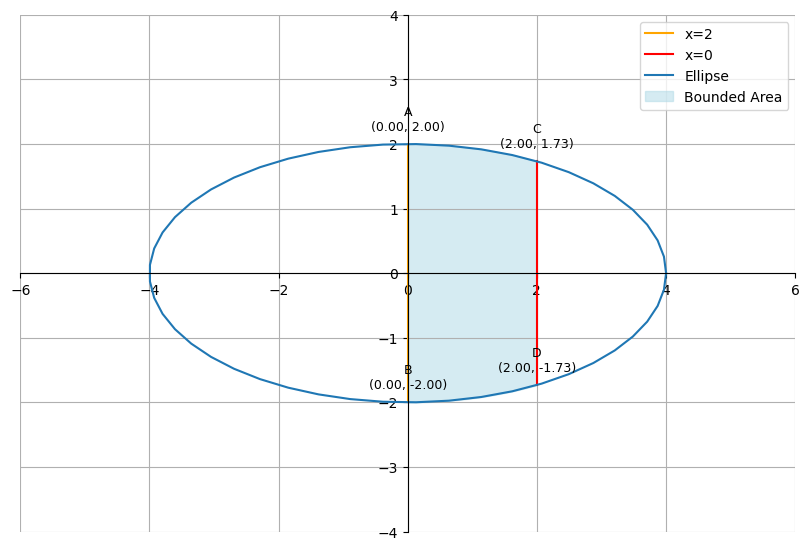
\includegraphics[width=1\textwidth]{plots/plot.png}
    \caption{Intersection of line and ellipse}
    \label{fig:plot}
\end{figure}  
}
\end{document}
